%%%%%%%%%%%%%%%%%%%%%%%%%%%%%%%%%%%%%%%%%%%%%%%%%%%%%%%%%%%%%%%%%%%%%%%%%%%%%%%%
%2345678901234567890123456789012345678901234567890123456789012345678901234567890
%        1         2         3         4         5         6         7         8

\documentclass[letterpaper, 10 pt, conference]{ieeeconf}
\IEEEoverridecommandlockouts
\overrideIEEEmargins

% See the \addtolength command later in the file to balance the column lengths
% on the last page of the document

%%%%%%%%%%%%%%%%%%%%%%%%%%%%%%%%%%%%%%%%%%%%%%%%
\usepackage[english]{babel}
\selectlanguage{english}

\usepackage{amsfonts}
\usepackage{amsmath}
\usepackage{amssymb}

\DeclareMathOperator*{\argmin}{arg\,min}
\DeclareMathOperator*{\argmax}{arg\,max}

\usepackage{graphicx}
\DeclareGraphicsExtensions{.pdf,.eps,.png,.jpg}
\graphicspath{{./fig/}}
\usepackage{booktabs}
\usepackage[font=footnotesize]{subcaption}
\usepackage[font={footnotesize}]{caption}

\usepackage{tikz}
\usepackage{tikzscale}
\usepackage{gnuplot-lua-tikz}

\newcommand{\includetexfig}[1]{\input{fig/#1.tex}}

\usetikzlibrary{shapes,fit,positioning}

\tikzstyle{state}=[circle,draw,thick]
\tikzstyle{observation}=[regular polygon,regular polygon sides=4,inner sep=1pt,draw,thick]

\tikzstyle{edata}=[draw,thick,rounded corners,minimum height=.7cm,text width=1.5cm,align=center]
\tikzstyle{data}=[above,text width=1.5cm,align=left]
\tikzstyle{process}=[rectangle,draw,thick,minimum height=.7cm,text width=1.5cm,align=center]
\tikzstyle{io}=[]

\newcommand{\crefrangeconjunction}{--}
\usepackage[capitalize]{cleveref}
%%%%%%%%%%%%%%%%%%%%%%%%%%%%%%%%%%%%%%%%%%%%%%%%

\title{\LARGE \bf
Multimodal Object Recognition from Visual and Audio Sequences%
}

\author{Weipeng He, Haojun Guan and Jianwei Zhang%
\thanks{W. He, H. Guan and J. Zhang are with TAMS, Department of Informatics, University of Hamburg, Vogt-K\"olln-Str. 30, 22527 Germany. {\tt\small 2he,guan,zhang@informatik.uni-hamburg.de}}%
}

\begin{document}

\maketitle
\thispagestyle{empty}
\pagestyle{empty}

%%%%%%%%%%%%%%%%%%%%%%%%%%%%%%%%%%%%%%%%%%%%%%%%%%%%%%%%%%%%%%%%%%%%%%%%%%%%%%%%
\begin{abstract}
This paper describes a visual-audio object recognition system using hidden Markov models. The system uses the bag-of-words model with scale invariant feature transform descriptors as the visual feature and the mel-frequency cepstrum coefficients as the audio feature. The classification of objects is based on computing the probabilities with learned hidden Markov models. Two different fusion methods are used in the system: feature fusion and decision fusion. The former method learns a joint probability distribution with one HMM, while the latter method learns two separate distributions for each modality and combines them under the conditional independence assumption. Experiments based on a dataset of 33 different household objects are carried out to evaluate the performance of these two fusion methods as well as unimodal approaches. The result shows that both fusion methods outperform unimodal methods, while these two methods are mostly comparable.
\end{abstract}

%%%%%%%%%%%%%%%%%%%%%%%%%%%%%%%%%%%%%%%%%%%%%%%%%%%%%%%%%%%%%%%%%%%%%%%%%%%%%%%%
\section{Introduction}
Humans not only use vision for object recognition, but also perceptions of other modalities, such as auditory, haptic and olfactory perceptions. These extra perceptions provide complementary information. This idea of multimodal object recognition can also be applied to robotic systems.

Traditional object recognition systems, which are exclusively based on visual information, are limited in several ways. They are sensitive to a number of image transformations such as view point change, occlusion and lighting variation. There are also cases where the visual information alone is not sufficient to distinguish an object. For example, a paper cup might have the same appearance as a ceramic cup, and it is difficult to distinguish them only by vision. However, if we strike or touch them, we can get auditory or haptic feedback from which it is possible to tell the difference.

Recent advances in robotics make it possible for robots to interact with objects and hence acquire multimodal information for object recognition. The study of how to use multimodal information for object recognition has become an important research topic.

Previously, there were studies using multimodal information for object recognition or object categorization. Sinapov et al.~\cite{sinapov_object_2011}\cite{sinapov_learning_2014} proposed a behavior-grounded relational learning method for multimodal object recognition. Their system used visual, audio and proprioceptive information collected by an upper-torso humanoid robot. Besides multimodal object recognition, Nakamura et al.~\cite{nakamura_multimodal_2007}\cite{nakamura_bag_2012} proposed unsupervised methods for multimodal object categorization based on visual, audio and haptic information.

The specific objective of this study is to build an object recognition system based on visual and audio information from videos of interactions with objects. To achieve such a goal, three basic questions need to be answered:
\begin{enumerate}
  \item What kind of features does the system use to represent the visual and audio information? The type of feature plays a critical role in the whole system. Good features make the learning trivial and bad features make the learning impossible.
  \item How does the system make classifications? Since an interaction is in essence perceived as images and sound which vary over time, we need a classification model that accounts for such time series data.
  \item How does the system combine multimodal information? A proper way to fuse multimodal information should favor reliable signals and avoid the influence of noisy signals.
\end{enumerate}

In the rest of this paper, we will address the answers to these questions.

\section{Feature Extraction}
According to the state-of-the-art features used in related applications, we choose the bag-of-words model with scale invariant feature transform (SIFT) descriptors as the visual feature and the mel-frequency cepstrum coefficients (MFCCs) as the audio feature for the system.

\subsection{Visual Feature}
The bag-of-words (BoW) model with SIFT descriptors is effective in representing the visual features of objects among the same category \cite{csurka_visual_2004,sivic_discovering_2005}. The application of bag-of-words models has achieved satisfying performance in visual object category recognition. Therefore, we use the bag-of-words model as the visual feature. The visual processing pipeline is shown in \cref{fig:vpipe}.

\begin{figure}[t]
  \footnotesize
  \centering
  \includegraphics[width=\linewidth]{vpipe.tikz}
  \caption{The visual processing pipeline.}
  \label{fig:vpipe}
\end{figure}

First, the image frames from the raw video are taken at a  frame rate of 5 frames per second. For each image frame, the keypoints are detected using the difference-of-Gaussian keypoint detector. Then, the SIFT descriptors of all the keypoints are computed (as described in \cite{lowe_distinctive_2004}). All the descriptors are quantized using a codebook of visual descriptors, which is prepared in advance. After that, the number of occurrences of the visual ``words'' are counted and represented as a normalized histogram (i.e. the bag-of-words feature). The codebook used in the experiment contains 20 ``words'', thus the visual feature is a sequence of 20-dimensional vectors.

\subsection{Audio Feature}
The mel-frequency cepstrum coefficients (MFCCs) are a kind of spectral feature of audio data. They encode interpretation of sounds similar to human perception. MFCCs have been commonly used for speech recognition, speaker recognition as well as music information retrieval. Hence, we choose MFCCs as the audio feature. The audio processing pipeline is shown in \cref{fig:apipe}.

\begin{figure}[t]
  \footnotesize
  \centering
  \includegraphics[width=\linewidth]{apipe.tikz}
  \caption{The audio processing pipeline.}
  \label{fig:apipe}
\end{figure}

The audio data are sampled at 8000 Hz. We first apply a shifting window with a window size of 2048 and shifting size of 1600 to get the audio frames, so that the rate of the audio frames is equal to that of the visual data. Then, for each audio frame, we calculate the MFCCs with 32 filter banks. Out of all the coefficients, the second to the 17th are taken and the rest is discarded, resulting in a 16-dimensional feature vector.

\section{Classification with HMM}
The hidden Markov model (HMM) is a statistical model for time series data, which have been well-known and widely used by researchers~\cite{rabiner_tutorial_1989}\cite{rabiner_fundamentals_1993}. The HMMs have been successfully applied to a number of research fields, including speech recognition~\cite{rabiner_fundamentals_1993}\cite{baker_dragon_1975}, image processing~\cite{chen_off-line_1994} and gesture recognition~\cite{mitra_gesture_2007}. As our object recognition system requires a learning model which can model time series data, the HMM is a perfect choice in this case. In addition to its wide usage, the HMM also allows us to estimate the probability, which can be used for further inference in modality fusion.

\subsection{Method}
Classification using HMM requires one model to be learned for each class $c$. The model for a class ($\lambda^c$) is learned to describe the distribution of all the instances of this class, that is:
\begin{equation}
  \lambda^c = \argmax_{\lambda} \prod_{\mathbf{x} \in D^c} P(\mathbf{x}|\lambda^c)
\end{equation}
in which $\mathbf{x}$ is the observation sequence ($\mathbf{x} = x_1 x_2 \cdots x_T$), and $D^c$ is the set of data instances the labels of which are $c$. The models are learned with the Baum-Welch algorithm. Then, when given a new instance of observation sequence, we can approximate the likelihood of a class with the learned model by
\begin{equation}
  P(\mathbf{x}|c) = P(\mathbf{x}|\lambda^c) .
\end{equation}

For a multiclass classification problem, the prediction of a new instance is carried out by choosing the class with the maximum likelihood:
\begin{equation}
  \label{eq:classif_s}
  f(\mathbf{x}) = \argmax_{c} P(\mathbf{x}|c) .
\end{equation}

For a binary classification problem, the classification is based on comparing the posterior probability to a given threshold $\theta$:
\begin{equation}
  \label{eq:classif_g}
  f(\mathbf{x}) =
  \left\{ \begin{array}{l l} +1, & \quad P(c=+1|\mathbf{x}) > \theta; \\ -1, & \quad \text{otherwise.}
  \end{array} \right.
\end{equation}

From Bayesian theory, the posterior probability of a class given the observation is
\begin{equation} \label{eq:posterior}
  P(c|\mathbf{x}) = \frac{P(\mathbf{x}|c)P(c)}{\sum_{c \in \{-1,+1\}} P(\mathbf{x}|c)P(c)}
\end{equation}
in which $P(c)$ is the prior probability of the class.

Considering the fact that randomly selecting objects as dataset is not likely to be the same as randomly drawing a sample in a real world, we notice that the prior probability is hard to estimate. However, if we assume that the prior probabilities are equal, we still can make the same decision by varying the threshold. We will later evaluate the performance of a classifier using the area under the receiver operating characteristic curve and such an evaluation method is not affected by the threshold. Therefore, by assuming equal prior probabilities, \cref{eq:posterior} can be rewritten as
\begin{equation}
  \label{eq:postsimp}
  P(c|\mathbf{x}) = \frac{P(\mathbf{x}|c)}{\sum_{c \in \{-1,+1\}} P(\mathbf{x}|c)} .
\end{equation}

As seen from \cref{eq:classif_s,eq:classif_g}, the key for both multiclass and binary classification is to know the likelihood $P(\mathbf{x}|c)$.

\subsection{Model Selection}
An important issue of HMM is selecting the model size and the observation distribution, i.e. the number of states, the number of components per state and the type of covariance matrix. The model choice can have a dramatic impact on the result.

Models with larger number of states and components are more complex. The covariance matrix can be either a full matrix or a diagonal matrix. The diagonal matrix assumes the feature coefficients are not correlated, thus is simpler than the full matrix.

\begin{table}[t]
  \caption{Comparison of simple and complex models.}
  \label{tab:model}
  \centering
  \begin{tabular}{p{.42\linewidth}p{.42\linewidth}}
    \toprule
    \multicolumn{1}{c}{\bfseries Simple Models} & \multicolumn{1}{c}{\bfseries Complex Models} \\ \midrule
    Smaller hypothesis space. & Larger hypothesis space. \\
    Easy to learn. & Hard to learn. \\
    Underfitting. & Overfitting. \\
    \bottomrule
  \end{tabular}
\end{table}

In general, simple models have a smaller hypothesis space, which means it is easy to learn. However, a smaller hypothesis space is less likely to contain target distribution, thus problems of underfitting can occur.

On the other hand, complex models have a larger hypothesis space, hence can better approximate the target distribution. However, since the Baum-Welch algorithm does not guarantee MLE, complex models are more prone to local optima. Furthermore, it could also result in overfitting if the training set is not large enough. The comparison of simple and complex models is listed in \cref{tab:model}.

The decision on the model choice should follow the principle of Occam's razor. Depending on different data, the best choice is the simplest model that can fit the data.

\section{Methods of Multimodal Fusion}
Having discussed how to extract feature vectors and how to make decisions based on it, we now move on to the final part of system design: multimodal signal fusion. The way to fuse the visual and audio information is essential to the object recognition system. A good method makes use of both modalities and avoids noises from unreliable signals.

Multimodal fusion methods may be classified into feature fusion, decision fusion and hybrid fusion according to the level of fusion ~\cite{atrey_multimodal_2010}. The feature fusion or early fusion is the approach of combining the multimodal features before they are sent as input of a learning model. The decision fusion or late fusion approach, on the other hand, analyzes each modality independently and then combines the individual decisions to a final result. The hybrid fusion is a combination of the two approaches.

The system incorporates two different designs regarding the fusion method: one with feature fusion and the other with decision fusion. To ground our discussion, consider the problem of classification using HMM with visual and audio features. The observation is a combination of visual and audio features, that is $\mathbf{x} = (\mathbf{v}, \mathbf{a})$. To make a decision using \cref{eq:classif_s} or \cref{eq:classif_g}, we need to compute the joint likelihood $P(\mathbf{v},\mathbf{a}|c)$.

\subsection{Feature Fusion}
\begin{figure}[t]
  \footnotesize
  \centering
  \includegraphics[width=\linewidth]{featurefs.tikz}
  \caption[Block diagram of the feature fusion approach.]{Block diagram of the feature fusion approach. Features of different modalities are first combined at the feature fusion module and then the joint probability is computed directly with the HMM which is learned with the combined feature.}
  \label{fig:featuref}
\end{figure}

Feature fusion is a direct approach in which the system learns the HMM with the concatenated features. Therefore the joint likelihood can be approximated with
\begin{equation}
  P(\mathbf{v},\mathbf{a}|c) = P(\mathbf{v},\mathbf{a}|\lambda_{va}^c)
\end{equation}
in which $\lambda_{va}^c$ are the estimated bimodal HMM parameters. A block diagram of such an approach is shown in \cref{fig:featuref}.

The advantage of feature fusion is that it utilizes the correlation between modalities. Theoretically, if the HMM are properly chosen and well trained, the feature fusion approach can yield an optimal estimation of the joint likelihood. However, learning both modalities at the same time increases the hypothesis space and also increases the difficulty of estimating the optimal parameters of the HMM. Furthermore, the video and audio features are required to be synchronized in order to get a meaningful combined feature.

\subsection{Decision Fusion}
\begin{figure}[t]
  \footnotesize
  \centering
  \includegraphics[width=\linewidth]{decisionfs.tikz}
  \caption[Block diagram of the decision fusion approach.]{Block diagram of the decision fusion approach. Likelihoods of different modalities are first computed individually and then combined at the decision level under the conditional independence assumption.}
  \label{fig:decisionf}
\end{figure}

An alternative approach, the decision fusion, is learning separate HMMs and combining the likelihood at the decision level. If we assume the features of different modalities are conditionally independent given the class, the joint likelihood can be computed as
\begin{equation}
  P(\mathbf{v},\mathbf{a}|c) = P(\mathbf{v}|c) P(\mathbf{a}|c) = P(\mathbf{v}|\lambda_v^c) P(\mathbf{a}|\lambda_a^c)
\end{equation}
in which $\lambda_{v}^c$ and $\lambda_{a}^c$ are the estimated HMM parameters for visual and audio features, respectively. A block diagram of such an approach is shown in \cref{fig:decisionf}.

Rather than learning a complex HMM model, the decision fusion approach learns two simple models. Therefore it is more likely to get an optimal estimation of the HMM parameters. However, the fusion is based on the assumption of conditional independence, which sometimes does not hold in reality. In this case, the joint likelihood estimation will be biased.

The difference between feature fusion and decision fusion is summarized in \cref{tab:fusion}.

\begin{table}[t]
  \caption{Comparison of feature fusion and decision fusion.}
  \label{tab:fusion}
  \centering
  \begin{tabular}{p{.42\linewidth}p{.42\linewidth}}
    \toprule
    \multicolumn{1}{c}{\bfseries Feature Fusion} & \multicolumn{1}{c}{\bfseries Decision Fusion} \\ \midrule
    Correlation between modalities is utilized. & Independent assumption needs to be held. \\
    Models are complex. & Models are simple. \\
    Synchronization is necessary. & Synchronization is not necessary. \\
    \bottomrule
  \end{tabular}
\end{table}

\section{Experiment and Results}
Experiments based on a visual-audio object dataset were carried out to evaluate different object recognition methods. The methods include feature fusion, decision fusion, visual only and audio only approaches.

\subsection{Data}
The dataset consists of videos of interactions with 33 different objects. The objects include household objects such as boxes, mugs, glasses, bowls, cans and bottles. The materials of the objects range from ceramic to glass, paper, wood, metal and plastic. Some of the objects contain content.

The videos were taken from a webcam at a resolution of $640 \times 480$ pixels and frame rate of 10 frames per second. The sound was recorded from the microphone on the webcam at 16000 Hz. When recording, the object was placed in the center of the view and took up a dominant part of the image. There were a few objects in the background.

\begin{figure}[t]
  \centering
  \begin{subfigure}[b]{.8\linewidth}
    \centering
    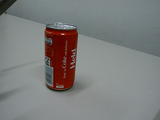
\includegraphics[width=.25\linewidth]{knock0} \hspace{.4cm}
    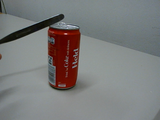
\includegraphics[width=.25\linewidth]{knock1} \hspace{.4cm}
    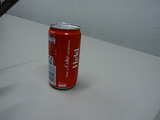
\includegraphics[width=.25\linewidth]{knock2}

    \includegraphics[width=\linewidth]{knock.tikz}
    \caption{Strike}
  \end{subfigure}

  \vspace{20pt}
  \begin{subfigure}[b]{.8\linewidth}
    \centering
    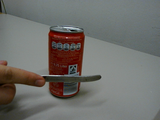
\includegraphics[width=.25\linewidth]{push0} \hspace{.4cm}
    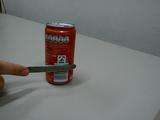
\includegraphics[width=.25\linewidth]{push1} \hspace{.4cm}
    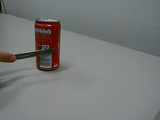
\includegraphics[width=.25\linewidth]{push2}

    \includegraphics[width=\linewidth]{push.tikz}
    \caption{Push}
  \end{subfigure}

  \vspace{20pt}
  \begin{subfigure}[b]{.8\linewidth}
    \centering
    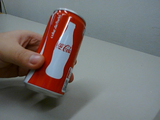
\includegraphics[width=.25\linewidth]{shake0} \hspace{.4cm}
    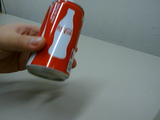
\includegraphics[width=.25\linewidth]{shake1} \hspace{.4cm}
    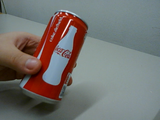
\includegraphics[width=.25\linewidth]{shake2}

    \includegraphics[width=\linewidth]{shake.tikz}
    \caption{Shake}
  \end{subfigure}
  \caption[Interactions with objects.]{Interactions with objects. The images are the video frames during the interaction. The figure below the images is the spectrogram of the sound during the interaction.}
  \label{fig:interaction}
\end{figure}

Three different interactions, including \emph{strike}, \emph{push} and \emph{shake}, were performed by the experimenter. The example videos of the interactions are shown in \cref{fig:interaction}. Some of the interactions produced sound, while the others did not. Each combination of object and interaction is recorded multiple times from different view points.

Each object is given a set of labels indicating whether this object belongs to a category. Six categories are studied in the experiment, including \emph{mugs}, \emph{bottles}, \emph{plastic objects}, \emph{metal objects}, \emph{fragile objects} and \emph{containers with content}. \Cref{tab:ocat} shows examples of these object categories.

\begin{table}
  \caption{Object categories.}
  \label{tab:ocat}
  \centering
  \begin{tabular}[t]{lc}
    \toprule
    \multicolumn{1}{c}{Category} & \multicolumn{1}{c}{Samples} \\ \midrule
    Mugs & \includegraphics[width=.1\linewidth]{object2} ~ 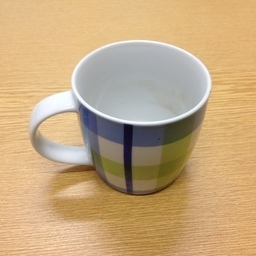
\includegraphics[width=.1\linewidth]{object3} ~ \includegraphics[width=.1\linewidth]{object6} \\
    Bottles & 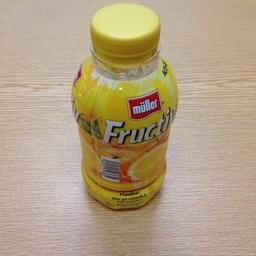
\includegraphics[width=.1\linewidth]{object16} ~ 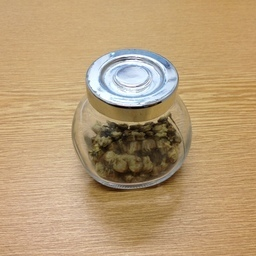
\includegraphics[width=.1\linewidth]{object19} ~ 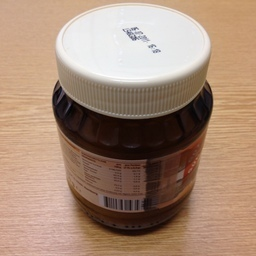
\includegraphics[width=.1\linewidth]{object20} \\
    Plastic & 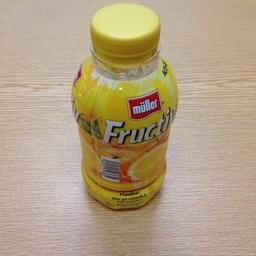
\includegraphics[width=.1\linewidth]{object16} ~ \includegraphics[width=.1\linewidth]{object17} ~ \includegraphics[width=.1\linewidth]{object33} \\
    Metal & \includegraphics[width=.1\linewidth]{object9} ~ \includegraphics[width=.1\linewidth]{object10} ~ \includegraphics[width=.1\linewidth]{object12} \\
    Fragile & \includegraphics[width=.1\linewidth]{object1} ~ \includegraphics[width=.1\linewidth]{object2} ~ \includegraphics[width=.1\linewidth]{object7} \\
    Containers & 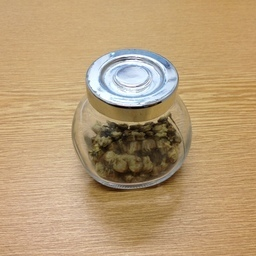
\includegraphics[width=.1\linewidth]{object19} ~ 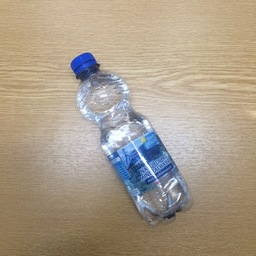
\includegraphics[width=.1\linewidth]{object24} ~ \includegraphics[width=.1\linewidth]{object29} \\
    \bottomrule
  \end{tabular}
\end{table}

\subsection{Evaluation}
The performances of the object recognition methods are evaluated for two different tasks: specific object recognition and generic category recognition.

\subsubsection{Specific Object Recognition}
The specific object recognition is the task of recognizing a particular object. For training, the system is presented with a set of objects with their labels. For testing, the system is shown a new video of a known object and needs to tell which object it is. The specific object recognition is posed as a multiclass classification problem, hence classification is based on \cref{eq:classif_s}.

The performance of each method for the specific object recognition is evaluated at an accuracy of 5-fold cross validation. The accuracy (ACC) is the percentage of correctly classified instances, namely
\[ \text{ACC} =  \frac{\text{\# correctly classified}}{\text{\# total}} . \]
For all methods, the HMM parameters are learned with two states, six mixture components for each state and diagonal covariance matrix.

\subsubsection{Generic Category Recognition}
The generic category recognition is the task of classifying an instance into a category or multiple categories. For training, the system is given a set of objects, some of which belong to a category (positive instances) and some of which do not (negative instances). Therefore, the task is posed as a binary classification problem and classified with \cref{eq:classif_g}.

For the generic category recognition task, we evaluate the classification performance with object-based validation. Each time the video instances of one object are separated from the whole dataset to be the test data and the rest are used for training. Therefore, all the test objects are always unseen objects, which are not in the training set. The HMM parameters are learned with various numbers of states, mixture components and diagonal covariance matrices. For each method, the model with the best performance is selected to represent the method.

In the case of generic category recognition, instead of accuracy we used the area under the receiver operating characteristic curve as the criterion. The accuracy does not comprehensively indicate the performance of a binary classifier. It is because there can be cases where more than 90 percent of the instances are negative and a trivial classifier which always predicts negative would result in a rather high accuracy.

Since the classification (\cref{eq:classif_g}) is based on a discrimination threshold, it is possible to use the receiver operating characteristic (ROC) curve to evaluate the classification result. The ROC curve is generated by plotting the true positive rate (TPR) against the false positive rate (FPR) by shifting the threshold from $0$ to $1$. The TPR, also known as recall rate or sensitivity, is the percentage of conditionally positive instances being predicted to be positive by the classifier:
\[ \text{TPR} =  \frac{\text{\# true positive}}{\text{\# conditional positive}} . \]
The FPR, also known as fall-out rate, is the percentage of conditionally negative instances being predicted to be positive by the classifier:
\[ \text{FPR} =  \frac{\text{\# false positive}}{\text{\# conditional negative}} . \]

The area under the ROC curve (AUC) can indicate the performance of a binary classifier. An AUC of a classifier is expected to be between $0.5$ and $1.0$, with larger value indicating better performance. The AUC of a random classifier is $0.5$ and that of a perfect classifier is $1.0$.

\section{Results}
\subsection{Specific Object Recognition Results}
The accuracy of each method for the specific object recognition task is shown in \cref{tab:spec}. The performance of both feature fusion and decision fusion methods is better than the visual only and audio only methods. There is an improvement of about $10\%$. These two fusion methods are only slightly different in performance.

\begin{table}
  \caption{Results of specific object recognition.}
  \label{tab:spec}
  \centering
  \begin{tabular}[h!]{lc}
    \toprule
    \multicolumn{1}{c}{Method} & Accuracy \\ \midrule
    Feature Fusion & \textbf{95.8\%} \\
    Decision Fusion  & 95.7\% \\
    Visual Only & 86.7\% \\
    Audio Only & 83.6\% \\
    \bottomrule
  \end{tabular}
\end{table}

\subsection{Generic Category Recognition Results}
The results of generic category recognition are shown in \cref{tab:cateory} and \cref{fig:catroc}. For recognition of mugs (\cref{fig:rocmug}), the decision fusion method has the best performance, followed closely by the visual only method and feature fusion method. For recognition of bottles and plastic objects (\cref{fig:rocbottle,fig:rocplastic}), both fusion methods are better than the unimodal methods. For recognition of metal objects (\cref{fig:rocmetal}), the visual only method is the best and the fusion methods are slightly worse. For recognition of fragile objects (\cref{fig:rocfragile}), the audio only method achieves a rather good performance while the visual only method is nearly random. In this case, the performance of both fusion methods are hurt by the visual signals. For recognition of containers with contents (\cref{fig:rocnonempty}), although all the methods performed poorly, there are improvements with the fusion methods.

On average, both fusion methods are better than the unimodal methods. What is interesting is that the two fusion methods are not only similar in AUC scores, but also their ROC curves appear close to each other. This indicates that they yield similar classification results.

\begin{table}
  \caption[Results of generic category recognition.]{Results of generic category recognition. The numbers are the AUC of different methods for the six object categories.}
  \label{tab:cateory}
  \centering
  \begin{tabular}[h]{l*{5}{p{.07\linewidth}}p{.11\linewidth}}
    \toprule
    & \multicolumn{6}{c}{Categories} \tabularnewline \cmidrule(r){2-7}
    \multicolumn{1}{c}{Method} & Mugs & Bottles & Plastic & Metal & Fragile & Containers \tabularnewline \midrule
    Feature Fusion & 0.750 & \textbf{0.802} & 0.820 & 0.830 & 0.711 & 0.671 \tabularnewline
    Decision Fusion & \textbf{0.771} & 0.798 & \textbf{0.839} & 0.870 & 0.697 & \textbf{0.675} \tabularnewline
    Visual Only & 0.763 & 0.778 & 0.813 & \textbf{0.877} & 0.590 & 0.567 \tabularnewline
    Audio Only & 0.642 & 0.707 & 0.732 & 0.772 & \textbf{0.819} & 0.620 \tabularnewline
    \bottomrule
  \end{tabular}
\end{table}

\begin{figure*}[t]
  \footnotesize
  \centering
  \begin{subfigure}[b]{.3\linewidth}
    \includegraphics[width=\linewidth]{mug.tikz}
    \caption{Mugs}
    \label{fig:rocmug}
  \end{subfigure}
  ~
  \begin{subfigure}[b]{.3\linewidth}
    \centering
    \includegraphics[width=\linewidth]{bottle.tikz}
    \caption{Bottles}
    \label{fig:rocbottle}
  \end{subfigure}
  ~
  \begin{subfigure}[b]{.3\linewidth}
    \includegraphics[width=\linewidth]{plastic.tikz}
    \caption{Plastic Objects}
    \label{fig:rocplastic}
  \end{subfigure}

  \begin{subfigure}[b]{.3\linewidth}
    \centering
    \includegraphics[width=\linewidth]{metal.tikz}
    \caption{Metal Objects}
    \label{fig:rocmetal}
  \end{subfigure}
  ~
  \begin{subfigure}[b]{.3\linewidth}
    \includegraphics[width=\linewidth]{fragile.tikz}
    \caption{Fragile Objects}
    \label{fig:rocfragile}
  \end{subfigure}
  ~
  \begin{subfigure}[b]{.3\linewidth}
    \centering
    \includegraphics[width=\linewidth]{nonempty.tikz}
    \caption{Containers with content}
    \label{fig:rocnonempty}
  \end{subfigure}
  \caption{ROC curves of generic category recognition results.}
  \label{fig:catroc}
\end{figure*}

\section{Conclusion and Future Work}
In this study, we have presented the design and implementation of a visual-audio object recognition system with hidden Markov models. The system has two different modality fusion methods: feature fusion and decision fusion. Experiments were carried out to evaluate the performance of these two methods and unimodal methods.

The results show that, for specific object recognition, both fusion methods increased the accuracy by about 10\%, compared to unimodal methods. For generic category recognition, both fusion methods increased the performance for most of the categories. Only if one of the input signals is too noisy, the result of the fusion methods will be worse than the result of the good signal.

The results of the experiments also show that, there is no significant difference between the two fusion methods. One possible explanation for this might be that the visual and audio signals are independent under the condition of being in one category.

It is recommended that further research be undertaken on the following aspects: building a real-time recognition system, increasing the size of the dataset and using multimodal signals for feature learning.

The current system cannot perform real-time recognition, for that the extraction of SIFT descriptors requires much computational power and the processing speed is about two frames per second. One possible solution is using SURF descriptors instead of SIFT.

The size of the dataset is critical to the system. With a large dataset it is possible to use discriminative methods to learn combination rules. For example, the reliabilities of the modalities can be estimated using a validation set taken from the training set. The reliabilities can be further used for modifying the influence of each signal. To increase the size of the dataset, it is possible to implement robotic systems to automatically collect data or acquire unlabeled data from Internet sources.

Although the performance of a multimodal object recognition system can be improved by finding the optimal combination rule, the upper bound of the performance is decided by the quality of the features. On the other hand, thinking of the properties of multimodal signals, for example that the signals appearing at the same time contain congruent semantic information, we can actually use the properties as a heuristic for unsupervised learning of good representation. Eventually, the better representation will improve the performance of the recognition system.

%%%%%%%%%%%%%%%%%%%%%%%%%%%%%%%%%%%%%%%%%%%%%%%%%%%%%%%%%%%%%%%%%%%%%%%%%%%%%%%%

\section*{ACKNOWLEDGMENT}
This work is supported and founded by the DFG German Research Foundation (grant \#1247) International Research Training Group CINACS (Cross-modal Interactions in Natural and Artificial Cognitive Systems).

%%%%%%%%%%%%%%%%%%%%%%%%%%%%%%%%%%%%%%%%%%%%%%%%%%%%%%%%%%%%%%%%%%%%%%%%%%%%%%%%

\bibliographystyle{IEEEtran}
\bibliography{thesis}

\end{document}

